\chapter{Métodos de Visualización Empleados}

En esta sección se discutirán los distintos métodos empleados, sobre cada uno de los gráficos, para analizar los datos seleccionados y elegir una técnica de reducción óptima para cada uno de los gráficos. Cada infograma es distinto al anterior, ya que representa información distinta y la estructura de diferente manera. Por eso no es posible aplicar las mismas técnicas sobre todos. Cada uno debe ser analizado específicamente para conocer cuáles son sus límites a la hora de dibujarlo, los tipos de datos que es capaz de representar y, que operaciones sobre los datos representan fielmente lo que quieren contar.

Los siguientes apartados se centrarán en explicar cómo funcionan cada uno de los gráficos disponibles en la API, que técnicas se han utilizado para reducir la cantidad de datos y resumirlos de forma que sean lo más representativos y, qué parámetros son necesarios indicarles para ejecutarlos. Todas las funciones se realizan mediante peticiones de tipo \textit{get}. Cabe destacar que cada uno de los gráficos que se generan son adaptativos a la resolución del dispositivo en el que se esté usando la API.

A continuación, se puede apreciar un listado con todos los gráficos disponibles en la API y que se explican en detalle posteriormente:
\begin{itemize}
	\item Histograma
	\item Boxplot
	\item Scatterplot
	\item Heatmap
	\item Bubble Chart
	\item Scatterplot Matrix
	\item Pie Chart
	\item Line Chart
	\item Stacked Area Chart
	\item Bar Chart
\end{itemize}

\section{Cuestiones generales sobre la visualización}
Como ya se ha explicado anteriormente, todo el sistema está desarrollado para funcionar sobre conjuntos de datos 'Big Data'. Esto conlleva que los cálculos sobre esos conjuntos de datos sea realmente la dificultad que tiene este proyecto. Para obtener una representación gráfica, por ejemplo un histograma o un boxplot, es necesario obtener unos valores calculados como máximo, mínimo, cuartiles, agrupaciones, conteo de datos, etc. Aquí es donde realmente está la complejidad de representar un histograma en comparación con otras herramientas clásicas, sobre conjuntos de datos de menor tamaño. 

Spark provee funcionalidad que permite calcular estas operaciones o parte de ellas de manera rápida y eficaz, pero lo interesante de este proyecto es la utilización de estas herramientas, para obtener los valores y a continuación, crear un gráfico representativo de lo que ocurre con el conjunto 'Big Data'.

En las siguientes secciones, se van a exponer cada uno de los gráficos implementados, explicando los pasos seguidos y los cálculos necesarios para dibujarlos.

\section{Histograma}
La idea del histograma es la de contabilizar los valores de una o varias columnas de un grupo de datos. Se pueden elegir la cantidad de agrupaciones o segmentos basados de los registros de los datos. Esta será la cantidad de columnas que tendrá el histograma. 

Una vez elegidos cuantos segmentos se necesitan, se calculan los limites de cada uno de ellos. Para ello, es necesario obtener el máximo y mínimo valor de todos los registros de los datos en la columna seleccionada, y aplicar la siguiente operación:

\begin{verbatim}
	(Máximo – Mínimo) / Número de segmentos = Amplitud de cada segmento
\end{verbatim}

Con la amplitud de cada uno de los segmentos, se obtienen los límites de cada uno, es decir, el máximo y mínimo valor de cada uno donde deben estar agrupados los valores. A continuación, se filtran los valores de las columnas seleccionadas y se contabilizan. Sólo queda guardar los resultados en JSON para su posterior representación gráfica.

Hay que tener en cuenta que el límite para elegir el número de segmentos son la cantidad de píxeles del gráfico en la pantalla, por esa razón se agrupan los valores a representar. Se puede ver un ejemplo en la figura \ref{fig:ejemplohistograma}
\begin{figure}
	\centering
	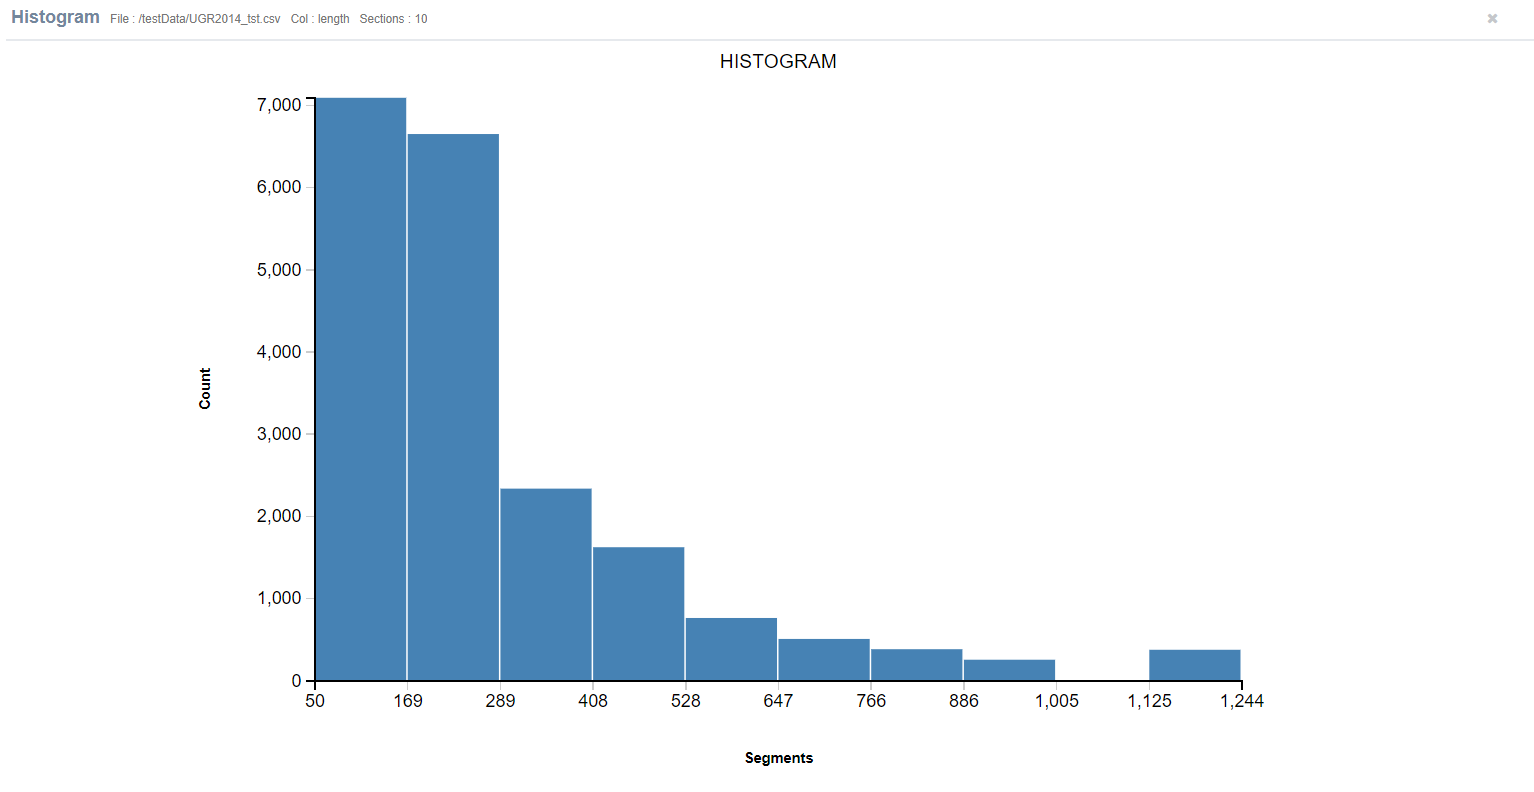
\includegraphics[width=1\linewidth]{imagenes/ejemplo_histograma}
	\caption{Ejemplo de un histograma}
	\label{fig:ejemplohistograma}
\end{figure}

Para la ejecución del histograma (ejemplo de URL\footnotemark), los parámetros por orden de inserción son:

\begin{tabular}{|l|l|p{7cm}|}
	\hline 
	\textbf{Campo} & \textbf{Tipo} & \textbf{Descripción} \\ 
	\hline \hline
	\multicolumn{3}{|c|}{\textit{Datos que proporciona la API}} \\
	\hline 
	MongoURL & String & URL del servidor MongoDB activo \\ 
	\hline 
	MongoDB & String & Base de datos dentro de MongoDB \\ 
	\hline 
	MongoCollect& String & Colección dentro de la base de datos en MongoDB \\ 
	\hline \hline
	\multicolumn{3}{|c|}{\textit{Datos que proporciona el usuario}} \\
	\hline 
	File & String & Fichero de entrada de datos, con formato CSV, situado en el HDFS (Hadoop) \\ 
	\hline 
	Col & String & Nombre de la columna del fichero de datos que se quiere analizar \\ 
	\hline 
	Sec & Number & Número de segmentos o intervalos en los que dividir los datos \\ 
	\hline 
\end{tabular} 

\footnotetext{/histogram?file=\%2FtestData\%2F1000\_ECBDL14\_10tst.csv\&col=f3\&sections=5}

\section{Boxplot}
El infograma boxplot se utiliza para representar las características principales de una distribución de valores. Estas características dan información acerca del comportamiento de los datos, en su conjunto, para una columna concreta del fichero. De cada uno de esas distribuciones o columnas de registros, lo primero es ordenar los datos de manera ascendente, para después calcular los siguientes valores:
\begin{itemize}
	\item Valor mínimo
	\item Primer cuartil
	\item Mediana
	\item Tercer cuartil
	\item Valor máximo
	\item IQR
\end{itemize}

Estas características son las que mejor representan el comportamiento de un conjunto de datos. El primer cuartil es el valor que para los que el 25\% de los valores ordenados son más pequeños que él. De manera opuesta, el tercer cuartil es el valor que representa que el 75\% de los valores son más pequeños. Después, la mediana representa el valor intermedio del conjunto de datos, lo que indica que el 50\% tienen valores más pequeños y el otro 50\% contiene registros mayores. El rango intercuartílico, o IQR, es la diferencia entre el tercer y primer cuartil del conjunto de datos. Sirve para eliminar algunos valores del conjunto que están extremadamente alejados y dispersos.

Spark implementa funciones específicas para calcular cada uno de estos valores sobre un Dataframe. Así, solo basta con utilizarlas para obtener los valores. Se puede ver un ejemplo en la figura \ref{fig:ejemploboxplot}
\begin{figure}
	\centering
	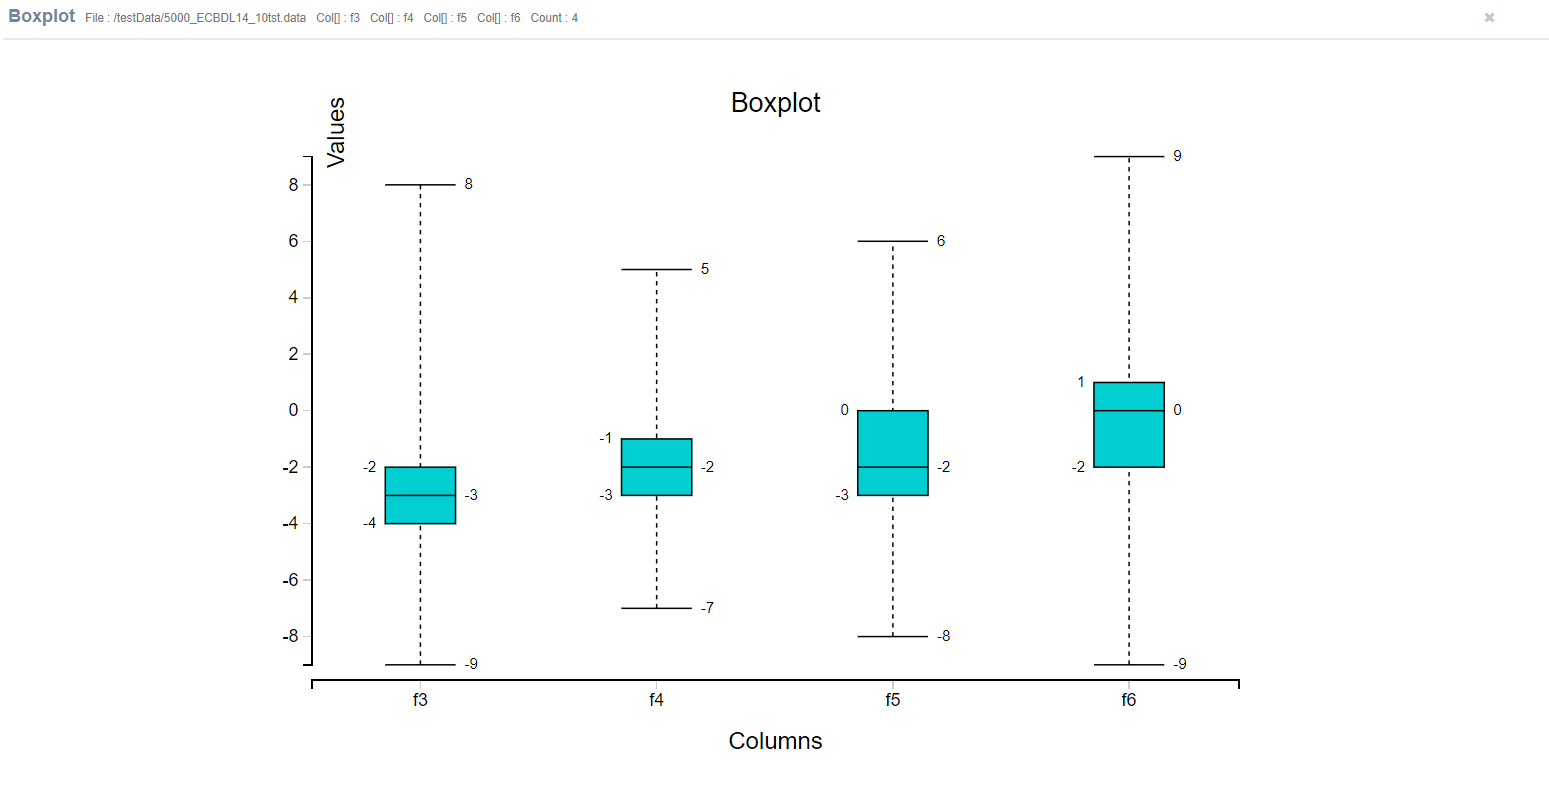
\includegraphics[width=1\linewidth]{imagenes/ejemplo_boxplot}
	\caption{Ejemplo del gráfico boxplot}
	\label{fig:ejemploboxplot}
\end{figure}

Para la ejecución del boxplot (ejemplo de URL\footnotemark), los parámetros por orden de inserción son:

\begin{tabular}{|l|l|p{7cm}|}
	\hline 
	\textbf{Campo} & \textbf{Tipo} & \textbf{Descripción} \\ 
	\hline \hline
	\multicolumn{3}{|c|}{\textit{Datos que proporciona la API}} \\
	\hline 
	MongoURL & String & URL del servidor MongoDB activo \\ 
	\hline 
	MongoDB & String & Base de datos dentro de MongoDB \\ 
	\hline 
	MongoCollect& String & Colección dentro de la base de datos en MongoDB \\ 
	\hline \hline
	\multicolumn{3}{|c|}{\textit{Datos que proporciona el usuario}} \\
	\hline 
	File & String & Fichero de entrada de datos, con formato CSV, situado en el HDFS (Hadoop) \\ 
	\hline 
	Count & Number & Numero de columnas del fichero a representar \\ 
	\hline 
	Col & Array[String] & Array con el nombre de las columnas del fichero seleccionadas \\ 
	\hline 
\end{tabular} 

\footnotetext{/boxplot?file=\%2FtestData\%2F1000\_ECBDL14\_10tst.csv\&count=3\&col=f3,f4,f5}

\section{Scatterplot}
El gráfico scatterplot está diseñado para representar pares de datos mediante puntos sobre un eje de coordenadas. Cada uno de los datos representa una posición sobre el eje correspondiente. Es una representación gráfica muy útil para averiguar si los datos siguen un determinado patrón, o por el contrario, simplemente no constata ningún comportamiento específico.

Aplicado al Big Data, reducir el número de datos a representar es fundamental, ya que dibujar todos y cada uno de los datos puede llegar a ser costoso y difícil de analizar su comportamiento. Dicho esto, es necesario buscar una solución de agrupación de los datos, sin perder información.

La técnica que se ha aplicado en este caso es dividir los ejes en secciones, de un tamaño variable, para que los datos estuvieran sobre una matriz. El siguiente paso ha sido averiguar en qué sección cae cada uno de los datos. Para hace esto de manera eficiente, se ha aplicado el siguiente algoritmo:
\begin{itemize}
	\item Se calcula el máximo y mínimo de cada uno de los ejes (grupo de datos)
	\item Obtenemos el tamaño de cada sección de la matriz por eje:
	\begin{verbatim}
		Tamaño de la sección = (Máximo – Mínimo) / Número de secciones
	\end{verbatim}
	\item Calculamos a que sección pertenece cada punto por eje:
	\begin{verbatim}
		Valor absoluto ((valor X - Mínimo) / Tamaño de la sección)
	\end{verbatim}
\end{itemize}

De esta manera, es posible saber en qué sección de la matriz cae cada uno de los puntos. Por último, contar cuantos puntos pertenecen a cada uno de las secciones de la matriz y calcular el centroide. Así, es posible reducir el número de datos a representar sin perder demasiada información de los mismos.

Como añadido, se ha insertado una gama de colores en la representación gráfica según la cantidad de puntos agrupados por secciones, para así facilitar la densidad de registros en ciertas zonas del gráfico.  Se puede ver un ejemplo en la figura \ref{fig:ejemploscatterplot}
\begin{figure}
	\centering
	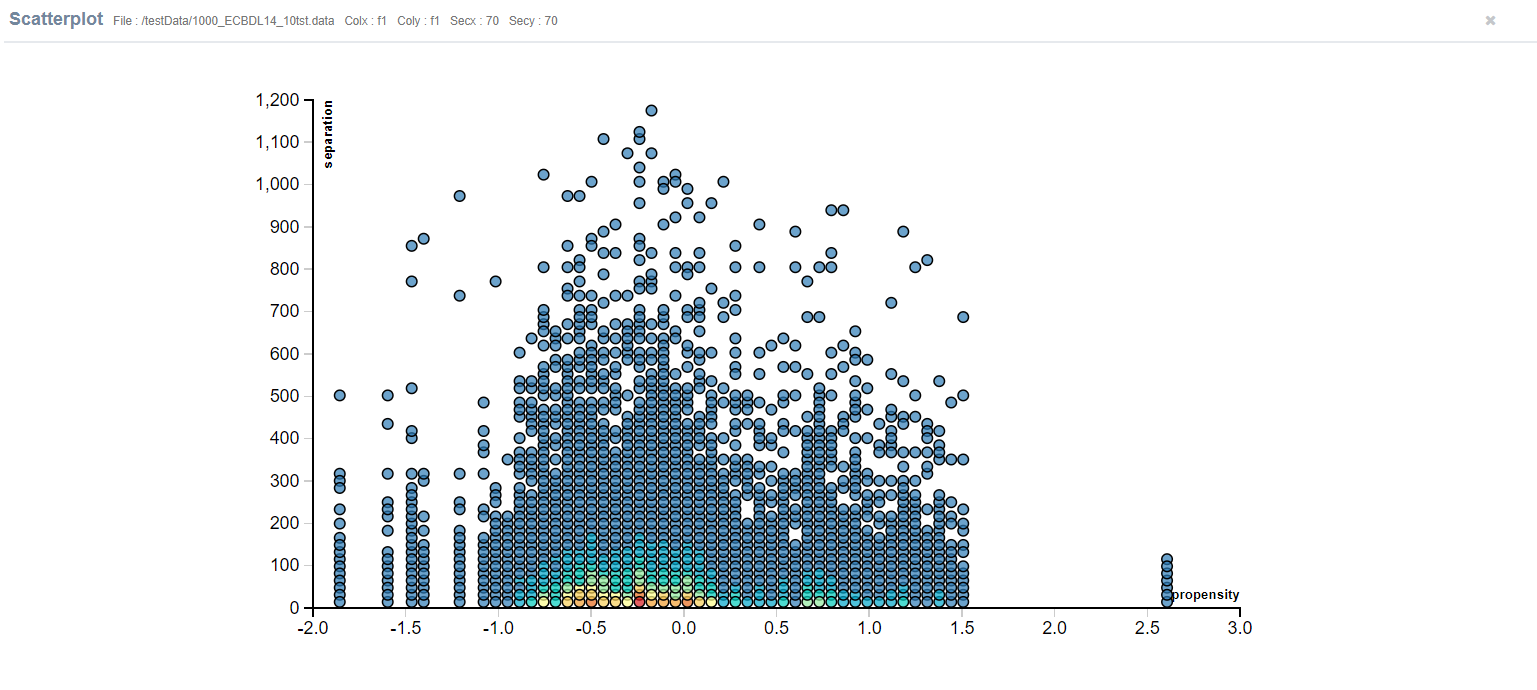
\includegraphics[width=1\linewidth]{imagenes/ejemplo_scatterplot}
	\caption{Ejemplo de scatterplot}
	\label{fig:ejemploscatterplot}
\end{figure}

Para la ejecución del scatterplot (ejemplo de URL\footnotemark), los parámetros por orden de inserción son:

\begin{tabular}{|l|l|p{7cm}|}
	\hline 
	\textbf{Campo} & \textbf{Tipo} & \textbf{Descripción} \\ 
	\hline \hline
	\multicolumn{3}{|c|}{\textit{Datos que proporciona la API}} \\
	\hline 
	MongoURL & String & URL del servidor MongoDB activo \\ 
	\hline 
	MongoDB & String & Base de datos dentro de MongoDB \\ 
	\hline 
	MongoCollect& String & Colección dentro de la base de datos en MongoDB \\ 
	\hline \hline
	\multicolumn{3}{|c|}{\textit{Datos que proporciona el usuario}} \\
	\hline 
	File & String & Fichero de entrada de datos, con formato CSV, situado en el HDFS (Hadoop) \\ 
	\hline 
	Colx & String & Columna de datos a representar como eje X \\ 
	\hline 
	Coly & String & Columna de datos a representar como eje Y \\ 
	\hline 
	Secx & Number & Número de secciones en el eje X para la matriz \\ 
	\hline 
	Secy & Number & Número de secciones en el eje Y para la matriz \\ 
	\hline 
\end{tabular} 

\footnotetext{/scatterplot?file=\%2FtestData\%2F1000\_ECBDL14\_10tst.csv\&colx=f3\&coly=f4\&secx=10\&secy=10}

\section{Heatmap}
El infograma Heatmap representa los datos en un formato de tabla con una gama de colores definida en base a una frecuencia u operación, desde colores que representan valores bajos hasta altos. Esta representación basada en colores hace que el gráfico sea mucho más fácil de entender y, por tanto, comprender mejor lo que indican los datos.

En la API, se seleccionan las columnas que van a representar los ejes X e Y, la columna de datos numéricos que calcular y el tipo de operación sobre dicha columna. Lo primero es agrupar los valores de las columnas seleccionados en variables de tipo ‘key-value’, tal que la clave esté formada por los valores de las columnas de los ejes, sin repeticiones, y el valor sea la columna elegida a representar, con la operación seleccionada aplicada, ya sea sumar, encontrar el valor máximo o encontrar el valor mínimo. Estas operaciones vienen implementadas por defecto en Spark para poder calcular estos valores. La dificultad del Big Data en este caso es que puede llegar a agruparse un número muy grande de registros, pero para ello también hay funciones de Spark que realizan estas agrupaciones, paralelizando el proceso, obteniendo más velocidad de cómputo.

Para los colores se ha aplicado la misma técnica que se utiliza en el gráfico Scatterplot.  Se puede ver un ejemplo en la figura \ref{fig:ejemploheatmap}
\begin{figure}
	\centering
	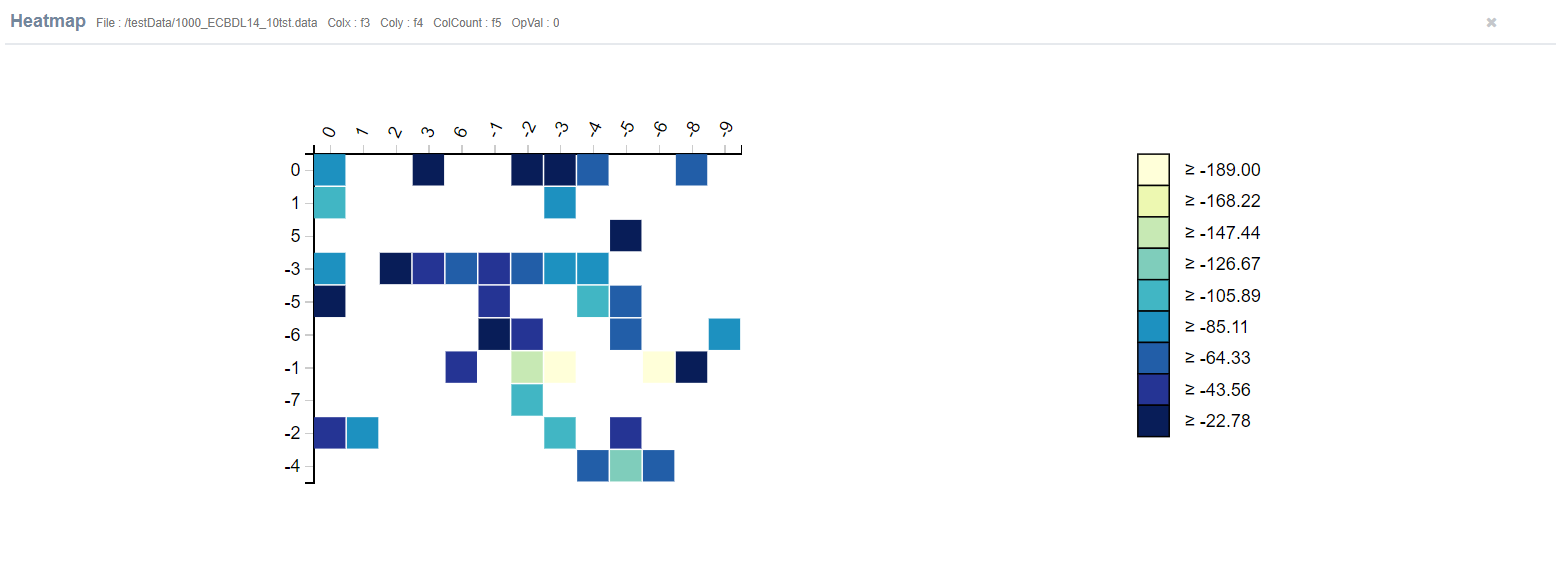
\includegraphics[width=1\linewidth]{imagenes/ejemplo_heatmap}
	\caption{Ejemplo de heatmap}
	\label{fig:ejemploheatmap}
\end{figure}

Para la ejecución del heatmap (ejemplo de URL\footnotemark), los parámetros por orden de inserción son:

\begin{tabular}{|l|l|p{7cm}|}
	\hline 
	\textbf{Campo} & \textbf{Tipo} & \textbf{Descripción} \\ 
	\hline \hline
	\multicolumn{3}{|c|}{\textit{Datos que proporciona la API}} \\
	\hline 
	MongoURL & String & URL del servidor MongoDB activo \\ 
	\hline 
	MongoDB & String & Base de datos dentro de MongoDB \\ 
	\hline 
	MongoCollect& String & Colección dentro de la base de datos en MongoDB \\ 
	\hline \hline
	\multicolumn{3}{|c|}{\textit{Datos que proporciona el usuario}} \\
	\hline 
	File & String & Fichero de entrada de datos, con formato CSV, situado en el HDFS (Hadoop) \\ 
	\hline 
	Colx & String & Columna de datos a representar como eje X \\ 
	\hline 
	Coly & String & Columna de datos a representar como eje Y \\ 
	\hline 
	Colcount & String & Columna de datos para representar el valor \\ 
	\hline 
	Opval & Number & Código de la operación para ser aplicada  [0-Sum, 1-Max, 2-Min] \\ 
	\hline 
\end{tabular} 

\footnotetext{/heatmap?file=\%2FtestData\%2F1000\_ECBDL14\_10tst.csv\&colx=f3\&coly=f4\&colCount=f5\&opVal=0}

\section{Bubble Chart}
El gráfico Bubble Chart está basado en el mismo algoritmo que el gráfico Scatterplot. Los datos se ejecutan de la misma forma que al aplicar el Scatterplot, cambiando únicamente la representación gráfica.

La diferencia principal del Bubble Chart es al representar los puntos del gráfico con tamaños diferentes, e incluso con colores diferentes, para enfatizar más la densidad de datos que se localizan en una zona concreta. Si hay muchos datos en una zona, aumenta el interés en esa zona y, por tanto, se representa con un círculo de mayor tamaño en comparación con otras zonas en las que existen menos puntos de datos.

Para calcular el tamaño de los círculos, se ha aplicado el mismo algoritmo que se utiliza para los colores en el gráfico Scatterplot, cambiando la densidad de puntos que se representa por un color, por un aumento en el radio del círculo.  Se puede ver un ejemplo en la figura \ref{fig:ejemplobubblechart}
\begin{figure}
	\centering
	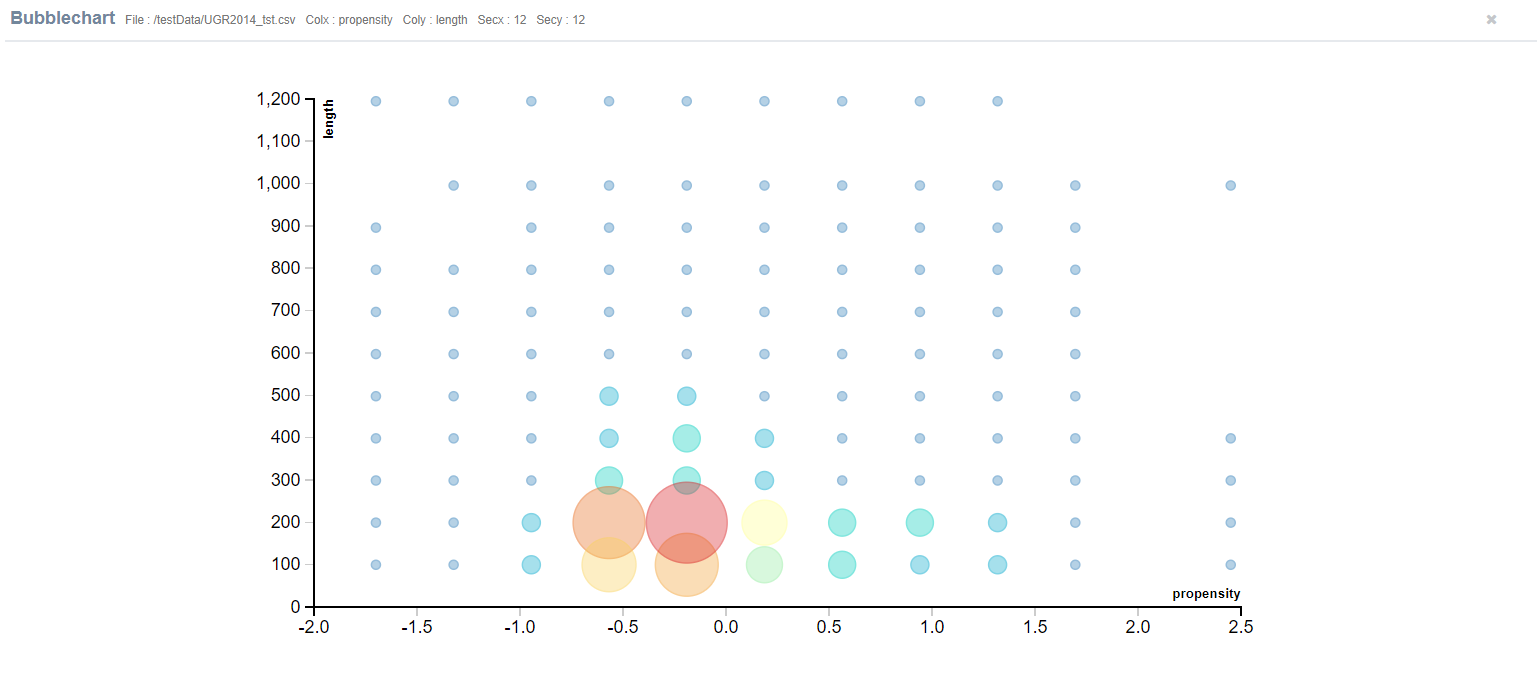
\includegraphics[width=1\linewidth]{imagenes/ejemplo_bubblechart}
	\caption{Ejemplo de un bubble chart}
	\label{fig:ejemplobubblechart}
\end{figure}

Para la ejecución del bubble chart (ejemplo de URL\footnotemark), los parámetros por orden de inserción son:

\begin{tabular}{|l|l|p{7cm}|}
	\hline 
	\textbf{Campo} & \textbf{Tipo} & \textbf{Descripción} \\ 
	\hline \hline
	\multicolumn{3}{|c|}{\textit{Datos que proporciona la API}} \\
	\hline 
	MongoURL & String & URL del servidor MongoDB activo \\ 
	\hline 
	MongoDB & String & Base de datos dentro de MongoDB \\ 
	\hline 
	MongoCollect& String & Colección dentro de la base de datos en MongoDB \\ 
	\hline \hline
	\multicolumn{3}{|c|}{\textit{Datos que proporciona el usuario}} \\
	\hline 
	File & String & Fichero de entrada de datos, con formato CSV, situado en el HDFS (Hadoop) \\ 
	\hline 
	Colx & String & Columna de datos a representar como eje X \\ 
	\hline 
	Coly & String & Columna de datos a representar como eje Y \\ 
	\hline 
	Secx & Number & Número de secciones en el eje X para la matriz \\ 
	\hline 
	Secy & Number & Número de secciones en el eje Y para la matriz \\ 
	\hline 
\end{tabular} 

\footnotetext{/bubblechart?file=\%2FtestData\%2F1000\_ECBDL14\_10tst.csv\&colx=f3\&coly=f4\&secx=10\&secy=10}

\section{Scatterplot Matrix}
El infograma Scatterplot Matrix es muy útil para determinar si existe algún tipo de correlación lineal entre un número determinado de variables. Saber que variables pueden contener alguna relación entre sí, o simplemente conocer que no aportan ningún tipo de información de valor, es de gran ayuda al analizar grandes cantidades de datos. El gráfico Scatterplot Matrix permite, de un solo vistazo, conocer esta información, para a continuación, entrar más en detalle con un Scatterplot sobre esas variables de interés.

Como ocurre con el gráfico Bubble Chart, el algoritmo para calcular cada uno de los cruces entre variables en el Scatterplot Matrix, es el mismo que el de Scatterplot. En esta ocasión, en vez de elegir dos columnas de los datos que representen cada uno de los ejes, se escogen un rango de variables que el usuario pueda conocer que sean de interés, y el algoritmo calculará cada uno de los cruces entre los mismos, con el fin de conocer si existe una correlación lineal entre varias. Se puede ver un ejemplo en la figura \ref{fig:ejemploscatterplotmatrix}
\begin{figure}
	\centering
	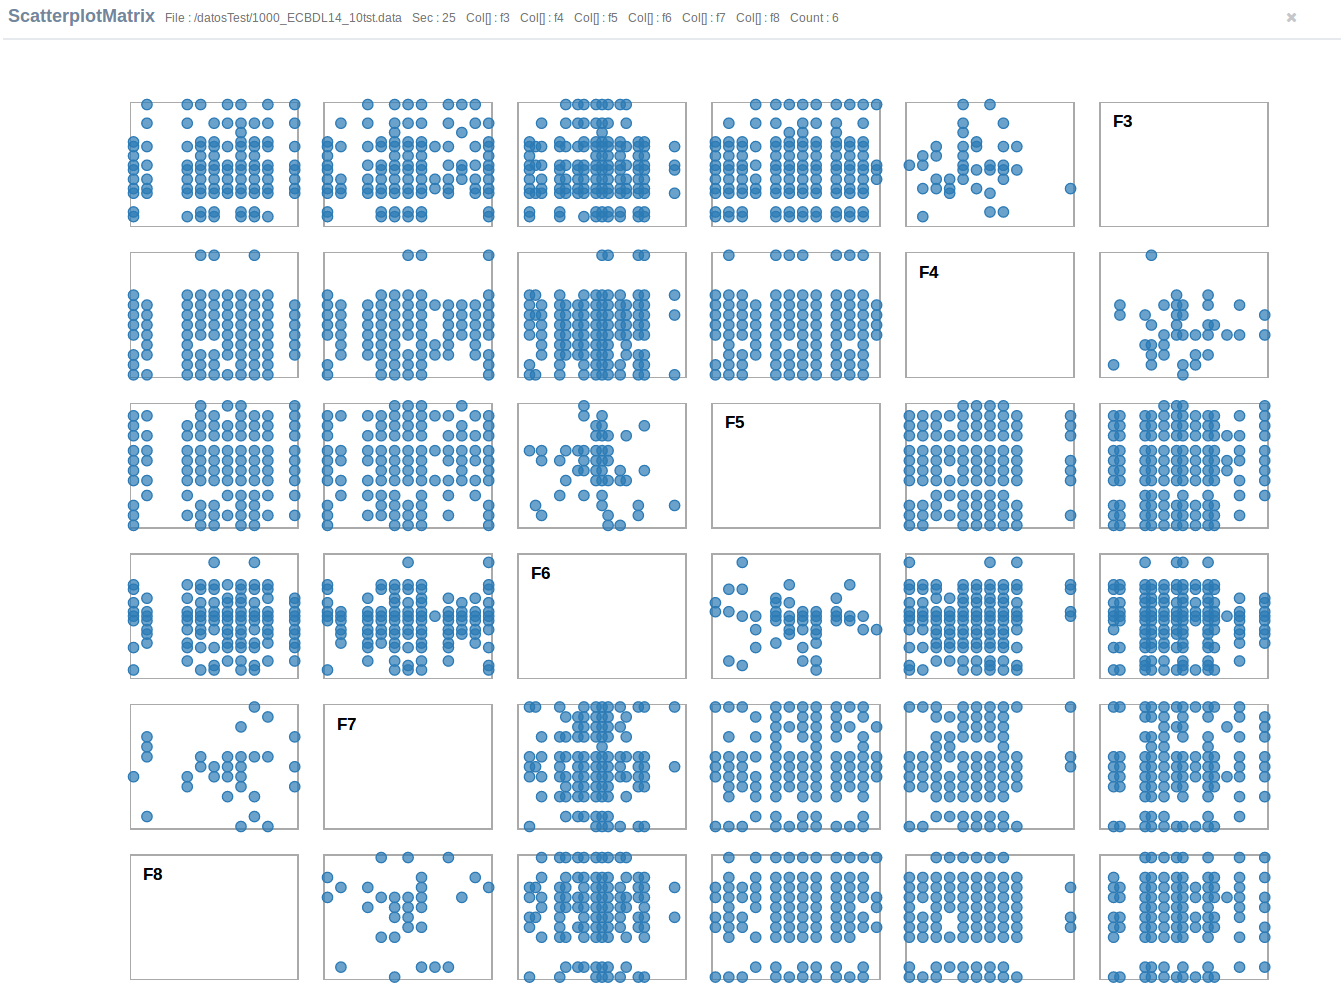
\includegraphics[width=1\linewidth]{imagenes/ejemplo_scatterplotMatrix}
	\caption{Ejemplo de scatterplot matrix}
	\label{fig:ejemploscatterplotmatrix}
\end{figure}

Para la ejecución del scatterplot matrix (ejemplo de URL\footnotemark), los parámetros por orden de inserción son:

\begin{tabular}{|l|l|p{7cm}|}
	\hline 
	\textbf{Campo} & \textbf{Tipo} & \textbf{Descripción} \\ 
	\hline \hline
	\multicolumn{3}{|c|}{\textit{Datos que proporciona la API}} \\
	\hline 
	MongoURL & String & URL del servidor MongoDB activo \\ 
	\hline 
	MongoDB & String & Base de datos dentro de MongoDB \\ 
	\hline 
	MongoCollect& String & Colección dentro de la base de datos en MongoDB \\ 
	\hline \hline
	\multicolumn{3}{|c|}{\textit{Datos que proporciona el usuario}} \\
	\hline 
	File & String & Fichero de entrada de datos, con formato CSV, situado en el HDFS (Hadoop) \\ 
	\hline 
	Sec & Number & Número de secciones sobre los ejes X e Y para la matriz \\ 
	\hline 
	Count & Number & Número de columnas seleccionadas a representar \\ 
	\hline 
	Col & Array[String] & Array con el nombre de las columnas del fichero seleccionadas \\ 
	\hline  
\end{tabular} 

\footnotetext{/scatterplotMatrix?file=\%2FtestData\%2F1000\_ECBDL14\_10tst.csv\&sec=5\&count=2\&col=f3,f4}

\section{Pie Chart}
El diagrama de sectores o Pie Chart, es un gráfico que consiste en dibujar un círculo dividido en sectores, en el que cada uno representa un valor de frecuencia de unos datos. Dicha frecuencia se dibuja aumentando el tamaño del sector dentro del círculo o disminuyéndolo. Por lo general, el gráfico Pie Chart suele representar valores cualitativos.

En la API, el algoritmo utilizado para realizar los cálculos ha sido agrupar los valores cualitativos de una variable seleccionada, de manera que no se repitan, junto con otra variable que represente la frecuencia de los distintos sectores. A cada uno de los valores cualitativos, se le asigna un sector del círculo, y el tamaño lo determina la variable de frecuencia seleccionada. Al igual que ocurre con el gráfico Heatmap, Spark proporciona métodos para agrupar valores en formato 'key-value' con las columnas seleccionadas. Como ha ocurrido en otros gráficos, se puede seleccionar una operación concreta que se desea aplicar sobre la variable de frecuencia. Las operaciones que se pueden seleccionar son de conteo, suma, máximo y mínimo.

Además, se ha añadido una leyenda con el nombre de los valores de los sectores y un color identificativo de cada uno de los sectores. Se puede ver un ejemplo en la figura \ref{fig:ejemplopiechart}
\begin{figure}
	\centering
	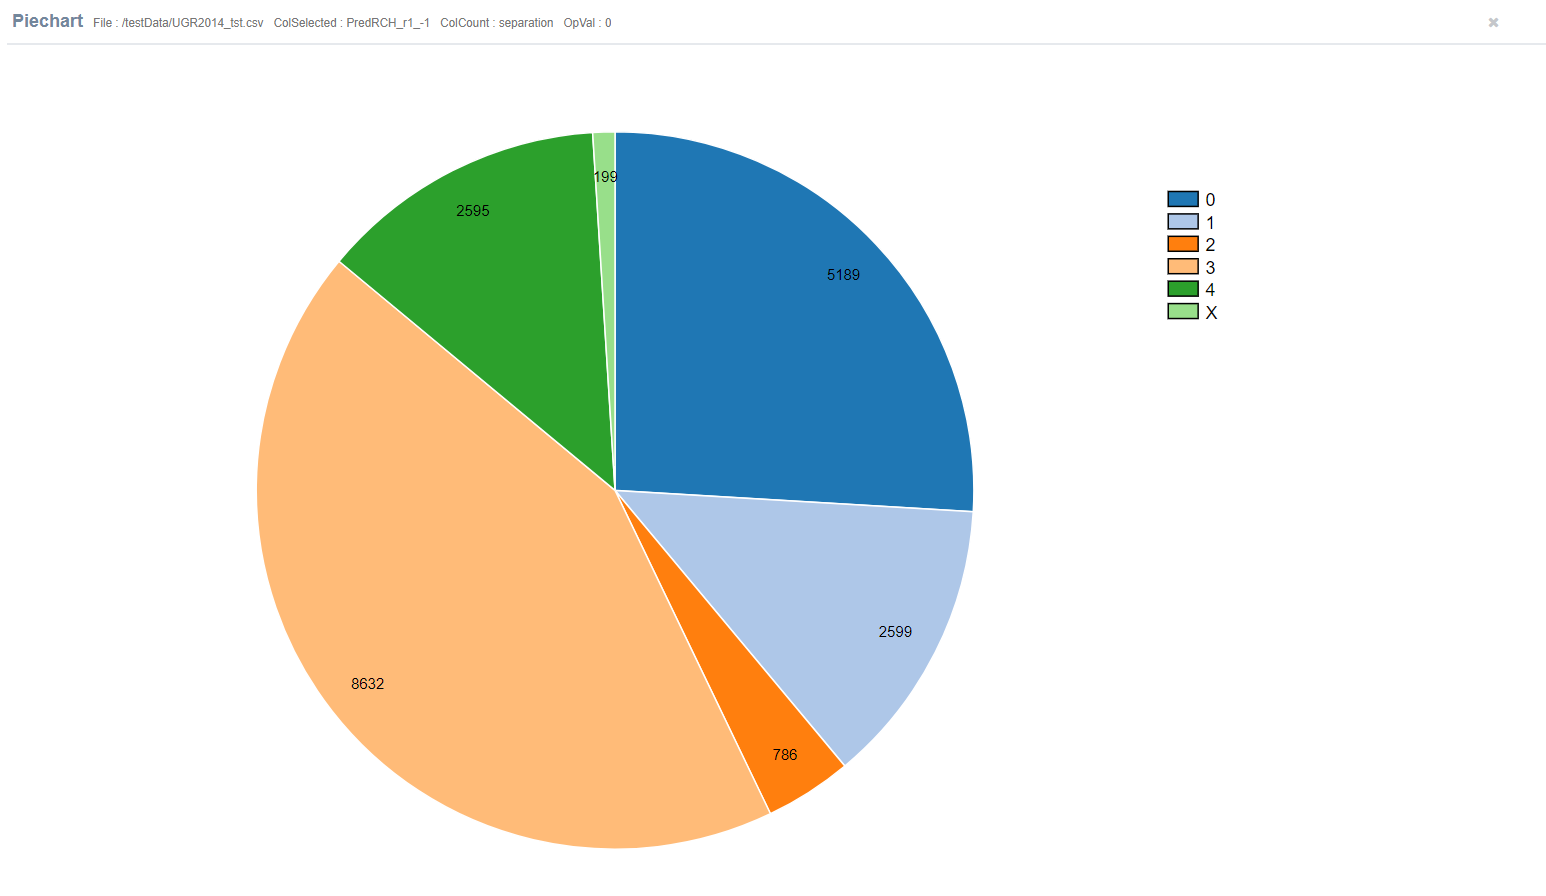
\includegraphics[width=1\linewidth]{imagenes/ejemplo_piechart}
	\caption{Ejemplo de pie chart}
	\label{fig:ejemplopiechart}
\end{figure}

Para la ejecución del pie chart (ejemplo de URL\footnotemark), los parámetros por orden de inserción son:

\begin{tabular}{|l|l|p{7cm}|}
	\hline 
	\textbf{Campo} & \textbf{Tipo} & \textbf{Descripción} \\ 
	\hline \hline
	\multicolumn{3}{|c|}{\textit{Datos que proporciona la API}} \\
	\hline 
	MongoURL & String & URL del servidor MongoDB activo \\ 
	\hline 
	MongoDB & String & Base de datos dentro de MongoDB \\ 
	\hline 
	MongoCollect& String & Colección dentro de la base de datos en MongoDB \\ 
	\hline \hline
	\multicolumn{3}{|c|}{\textit{Datos que proporciona el usuario}} \\
	\hline 
	File & String & Fichero de entrada de datos, con formato CSV, situado en el HDFS (Hadoop) \\ 
	\hline 
	Colselected & String & Columna que representa cada uno de los sectores del círculo \\ 
	\hline 
	Colcount & String & Columna que representa la variable de frecuencia de cada uno de los sectores \\ 
	\hline 
	Opval & Number & Código de la operación para ser aplicada [0-Count, 1-Sum, 2-Max, 3-Min] \\ 
	\hline  
\end{tabular} 

\footnotetext{/piechart?file=\%2FtestData\%2F1000\_ECBDL14\_10tst.csv\&colSelected=f3\&colCount=f4\&opVal=0}

\section{Line Chart}
Los gráficos de líneas representan una serie de puntos conectados por una línea, ajustados a una gran cantidad de datos mediante una sucesión consecutiva de valores, generalmente un periodo continuado de tiempo. Este gráfico es ideal para mostrar tendencias de los datos.

El algoritmo implementado para este gráfico se basa en subdividir los periodos de tiempo o un conjunto de valores que se representa en el eje X, y calcular el número de datos que caen dentro de cada una de las secciones. Es parecido al algoritmo que se utiliza en el Scatterplot solamente que en el LineChart se aplica sobre el eje X, pero no sobre el eje Y del gráfico. Una vez divididos los datos del eje X en sectores y asignados los puntos en cada uno de ellos, basta con calcular el punto medio entre ellos, para obtener un único punto en cada uno de las divisiones. Así, uniendo estos puntos, se obtiene como resultado la línea del gráfico.

Además, la API permite seleccionar un grupo de variables que representen una línea, componiendo así un gráfico de múltiples líneas comparativas, sobre la misma variable de valores continuos asociada al eje X. Se puede ver un ejemplo en la figura \ref{fig:ejemplolinechart}
\begin{figure}
	\centering
	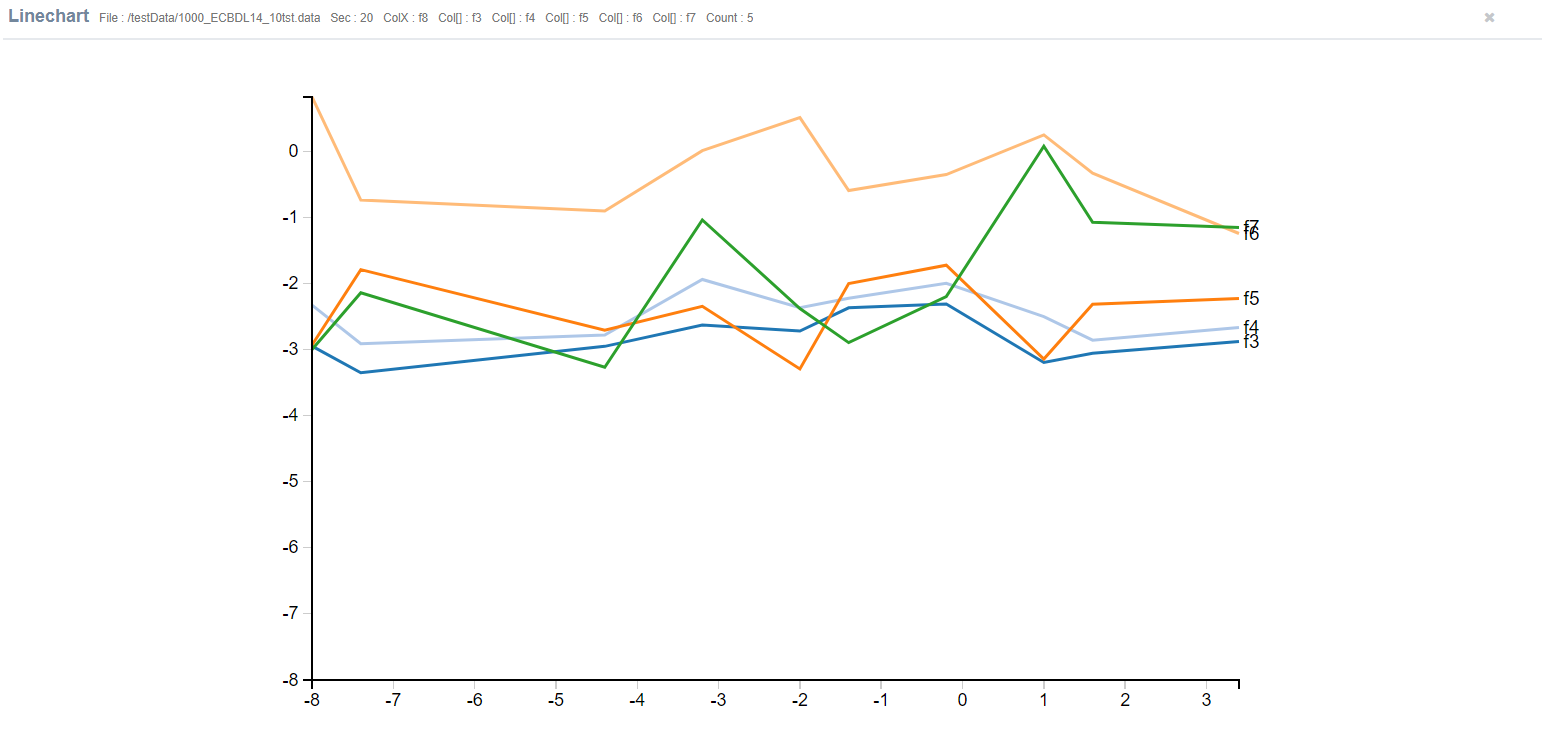
\includegraphics[width=1\linewidth]{imagenes/ejemplo_linechart}
	\caption{Ejemplo de line chart}
	\label{fig:ejemplolinechart}
\end{figure}

Para la ejecución del line chart (ejemplo de URL\footnotemark), los parámetros por orden de inserción son:

\begin{tabular}{|l|l|p{7cm}|}
	\hline 
	\textbf{Campo} & \textbf{Tipo} & \textbf{Descripción} \\ 
	\hline \hline
	\multicolumn{3}{|c|}{\textit{Datos que proporciona la API}} \\
	\hline 
	MongoURL & String & URL del servidor MongoDB activo \\ 
	\hline 
	MongoDB & String & Base de datos dentro de MongoDB \\ 
	\hline 
	MongoCollect& String & Colección dentro de la base de datos en MongoDB \\ 
	\hline \hline
	\multicolumn{3}{|c|}{\textit{Datos que proporciona el usuario}} \\
	\hline 
	File & String & Fichero de entrada de datos, con formato CSV, situado en el HDFS (Hadoop) \\ 
	\hline 
	Sec & Number & Número de secciones que dividir el eje X \\ 
	\hline 
	Colx & String & Columna que represente los valores continuos del eje X \\ 
	\hline 
	Count & Number & Número de columnas seleccionadas a representar por líneas \\ 
	\hline  
	Col & Array[String] & Array con el nombre de las columnas del fichero seleccionadas \\ 
	\hline
\end{tabular} 

\footnotetext{/linechart?file=\%2FtestData\%2F1000\_ECBDL14\_10tst.csv\&sec=10\&colX=f3\&count=2\&col=f4,f5}

\section{Stacked Area Chart}
El gráfico Stacked Area Chart utiliza una serie de variables con múltiples datos. Cada una de ellas comienza a partir de último punto sobre el eje X de la variable anterior. El gráfico representa todos los trazos de cada una de las variables acumuladas una sobre la otra. El Stacked Area Chart muestra las relaciones entre las distintas variables seleccionadas, ayudando a visualizar como contribuyen cada una al total acumulado.

El algoritmo para obtener los datos necesarios para pintarlo es el mismo que el aplicado en el Line chart. La diferencia está en la manera de visualizarlos, aportando otro tipo de información al usuario. Se puede ver un ejemplo en la figura \ref{fig:ejemplostackedareachart}

\begin{figure}
	\centering
	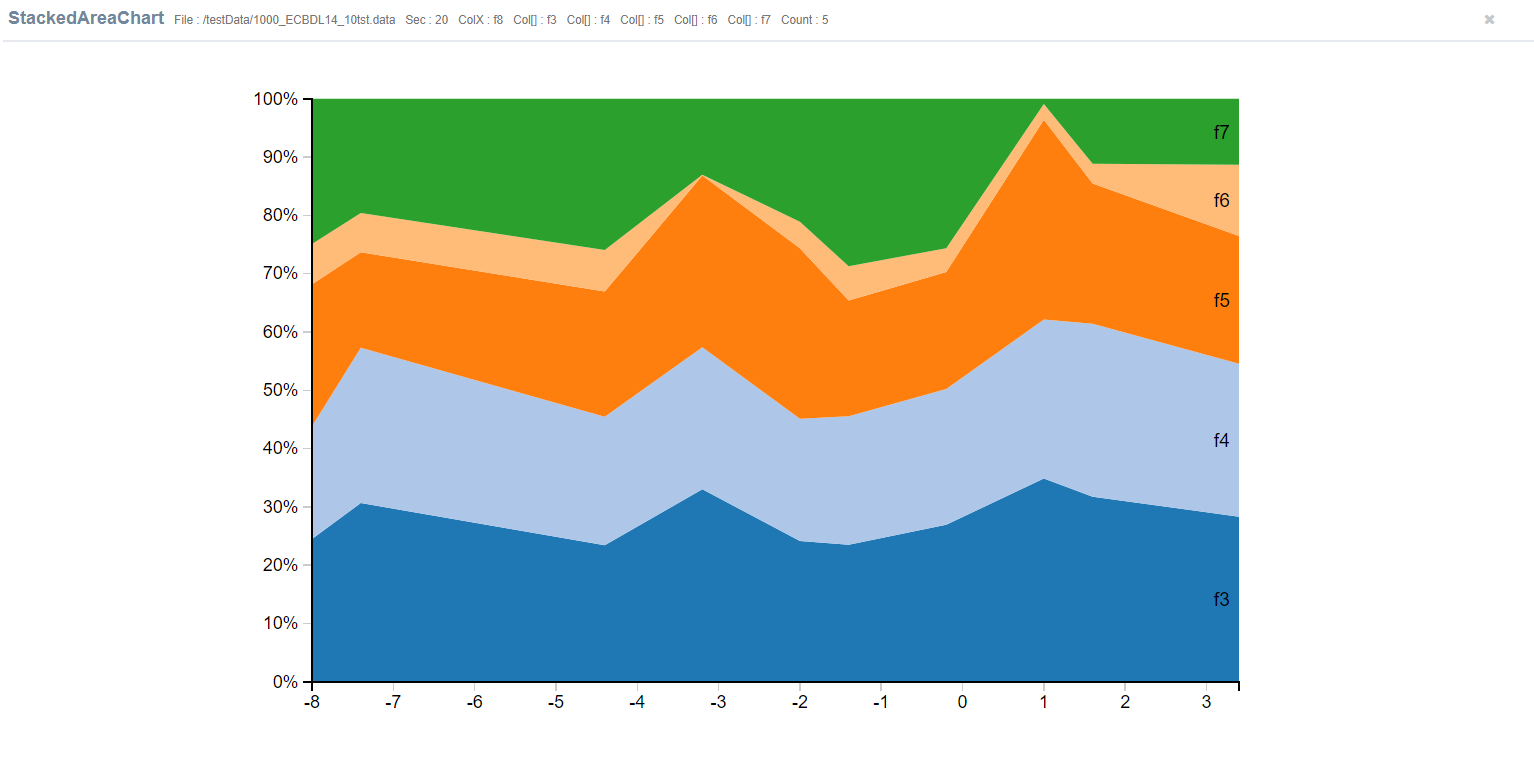
\includegraphics[width=1\linewidth]{imagenes/ejemplo_stackedareachart}
	\caption{Ejemplo de un stacked area chart}
	\label{fig:ejemplostackedareachart}
\end{figure}

Para la ejecución del stacked area chart (ejemplo de URL\footnotemark), los parámetros por orden de inserción son:

\begin{tabular}{|l|l|p{7cm}|}
	\hline 
	\textbf{Campo} & \textbf{Tipo} & \textbf{Descripción} \\ 
	\hline \hline
	\multicolumn{3}{|c|}{\textit{Datos que proporciona la API}} \\
	\hline 
	MongoURL & String & URL del servidor MongoDB activo \\ 
	\hline 
	MongoDB & String & Base de datos dentro de MongoDB \\ 
	\hline 
	MongoCollect& String & Colección dentro de la base de datos en MongoDB \\ 
	\hline \hline
	\multicolumn{3}{|c|}{\textit{Datos que proporciona el usuario}} \\
	\hline 
	File & String & Fichero de entrada de datos, con formato CSV, situado en el HDFS (Hadoop) \\ 
	\hline 
	Sec & Number & Número de secciones que dividir el eje X \\ 
	\hline 
	Colx & String & Columna que represente los valores continuos del eje X \\ 
	\hline 
	Count & Number & Número de columnas seleccionadas a representar por líneas \\ 
	\hline  
	Col & Array[String] & Array con el nombre de las columnas del fichero seleccionadas \\ 
	\hline
\end{tabular} 

\footnotetext{/stackedAreaChart?file=\%2FtestData\%2F1000\_ECBDL14\_10tst.csv\&sec=10\&colX=f3\&count=2\&col=f4,f5}

\section{Bar Chart}
Un gráfico Bar Chart resume un grupo de variables de tipo cuantitativas, usando otra variable que represente un valor numérico. Gráficamente, este valor representa la altura de cada una de las barras, teniendo información visual sobre la comparativa entre las distintas variables cuantitativas de cada una de las barras. Probablemente sea el gráfico más sencillo, pero a su vez el que más información aporta sobre el comportamiento de los datos subyacentes. 

Para el Bar Chart, se ha utilizado el mismo algoritmo que se ha implementado para el Pie Chart. Utiliza una variable o columna que representa cada uno de los valores del eje Y, agrupados para evitar repetición, sobre otra columna numérica a la que se le aplica una de las operaciones disponibles, las mismas que se pueden aplicar sobre el Pie Chart. Destacar que el gráfico se representa de manera horizontal, para representar en barras un mayor número de variables. Se puede ver un ejemplo en la figura \ref{fig:ejemplobarchart}
\begin{figure}
	\centering
	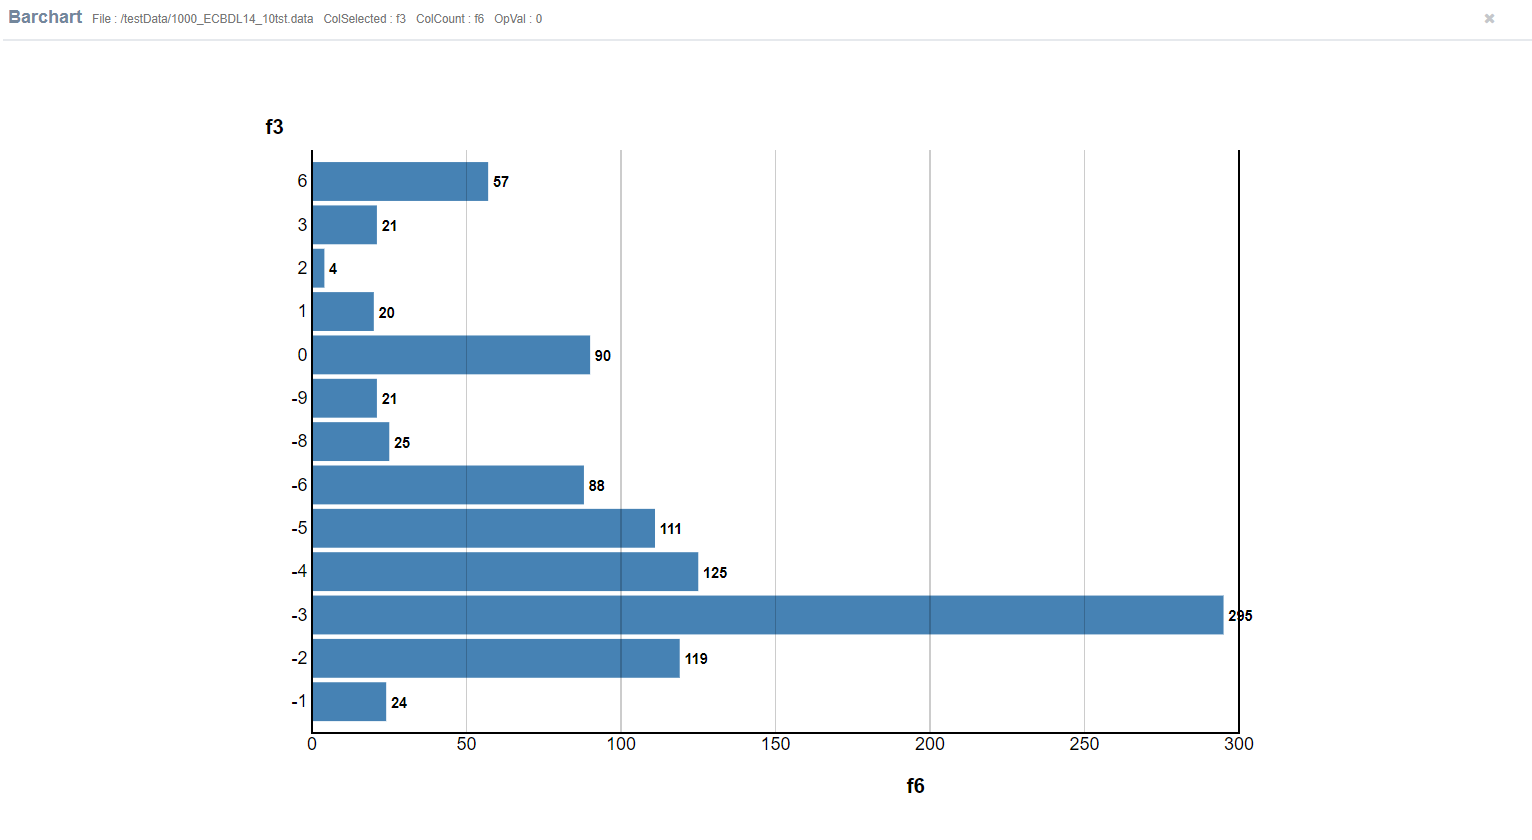
\includegraphics[width=1\linewidth]{imagenes/ejemplo_barchart}
	\caption{Ejemplo de bar chart}
	\label{fig:ejemplobarchart}
\end{figure}

Para la ejecución del bar chart (ejemplo de URL\footnotemark), los parámetros por orden de inserción son:

\begin{tabular}{|l|l|p{7cm}|}
	\hline 
	\textbf{Campo} & \textbf{Tipo} & \textbf{Descripción} \\ 
	\hline \hline
	\multicolumn{3}{|c|}{\textit{Datos que proporciona la API}} \\
	\hline 
	MongoURL & String & URL del servidor MongoDB activo \\ 
	\hline 
	MongoDB & String & Base de datos dentro de MongoDB \\ 
	\hline 
	MongoCollect& String & Colección dentro de la base de datos en MongoDB \\ 
	\hline \hline
	\multicolumn{3}{|c|}{\textit{Datos que proporciona el usuario}} \\
	\hline 
	File & String & Fichero de entrada de datos, con formato CSV, situado en el HDFS (Hadoop) \\ 
	\hline 
	Colselected & String & Columna que representa cada uno de las barras del diagrama \\ 
	\hline 
	Colcount & String & Columna que representa la variable de frecuencia de cada uno de las barras \\ 
	\hline 
	Opval & Number & Código de la operación para ser aplicada [0-Count, 1-Sum, 2-Max, 3-Min] \\ 
	\hline  
\end{tabular} 

\footnotetext{/barchart?file=\%2FtestData\%2F1000\_ECBDL14\_10tst.csv\&colSelected=f3\&colCount=f4\&opVal=0}